\documentclass{article}
\usepackage{graphicx}
\usepackage{hyperref}
\usepackage{amsmath}
\usepackage{times}

\textwidth=6.2in
\textheight=8.5in
%\parskip=.3cm
\oddsidemargin=.1in
\evensidemargin=.1in
\headheight=-.3in


%------------------------------------------------------------
% newcommand
%------------------------------------------------------------
\newcommand{\scscst}{\scriptscriptstyle}
\newcommand{\scst}{\scriptstyle}
\newcommand{\Robject}[1]{{\texttt{#1}}}
\newcommand{\Rfunction}[1]{{\texttt{#1}}}
\newcommand{\Rclass}[1]{\textit{#1}}
\newcommand{\Rpackage}[1]{\textit{#1}}
\newcommand{\Rexpression}[1]{\texttt{#1}}
\newcommand{\Rmethod}[1]{{\texttt{#1}}}
\newcommand{\Rfunarg}[1]{{\texttt{#1}}}

\usepackage{Sweave}
\begin{document}
\Sconcordance{concordance:APA_template_tables.tex:APA_template_tables.Rnw:%
1 27 1 1 0 22 1 1 2 1 0 2 1 5 0 1 1 6 0 1 2 8 1 1 2 5 0 1 2 10 1 1 2 1 %
0 2 1 4 0 1 2 11 1 1 2 1 0 1 1 3 0 1 2 6 1 1 10 4 0 1 2 4 1 1 2 1 0 1 1 %
16 0 1 2 8 1 1 2 1 0 1 1 21 0 1 2 7 1 1 3 28 0 1 3 1 1}


%------------------------------------------------------------
\title{Simple example of Sweave}
%------------------------------------------------------------
\author{Aedin Culhane}
%\date{}





\maketitle
\tableofcontents


%-------------------------------------------
\section{Introduction}
%--------------------------------------------

Just a simple introduction to Sweave. 

\begin{Schunk}
\begin{Sinput}
> a=1
> b=4
> a+b
\end{Sinput}
\begin{Soutput}
[1] 5
\end{Soutput}
\begin{Sinput}
> print("hello")
\end{Sinput}
\begin{Soutput}
[1] "hello"
\end{Soutput}
\end{Schunk}

We can call R commands from the text. For example a+b= 5

%-------------------------------------------
\section{Including a Plot}
%--------------------------------------------
Now for a plot.  Note we include fig=TRUE, which prints the plot within the document


\begin{Schunk}
\begin{Sinput}
> plot(1:10, col="red", pch=19)
\end{Sinput}
\end{Schunk}
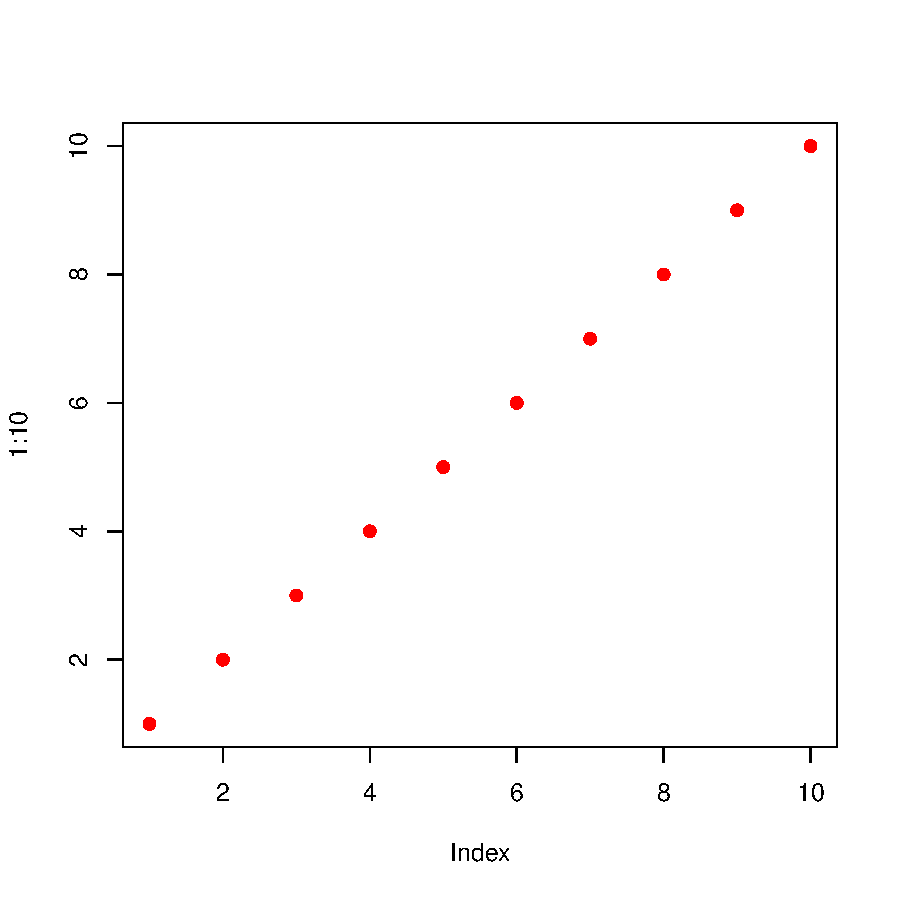
\includegraphics{Fig-test2}

Thats it.... simple hey!


%------------------------------------
\subsection{More on Plots}
%-------------------------------------

To make the plot a little nicer, we can add a caption. Also let's change the size of the plot to be 4" in height and 6" in width

\begin{figure}
\begin{Schunk}
\begin{Sinput}
> par(mfrow=c(1,2))
> plot(1:10, col="green", pch=21)
> barplot(height=sample(1:10,5), names=LETTERS[1:5], col=1:5)
\end{Sinput}
\end{Schunk}
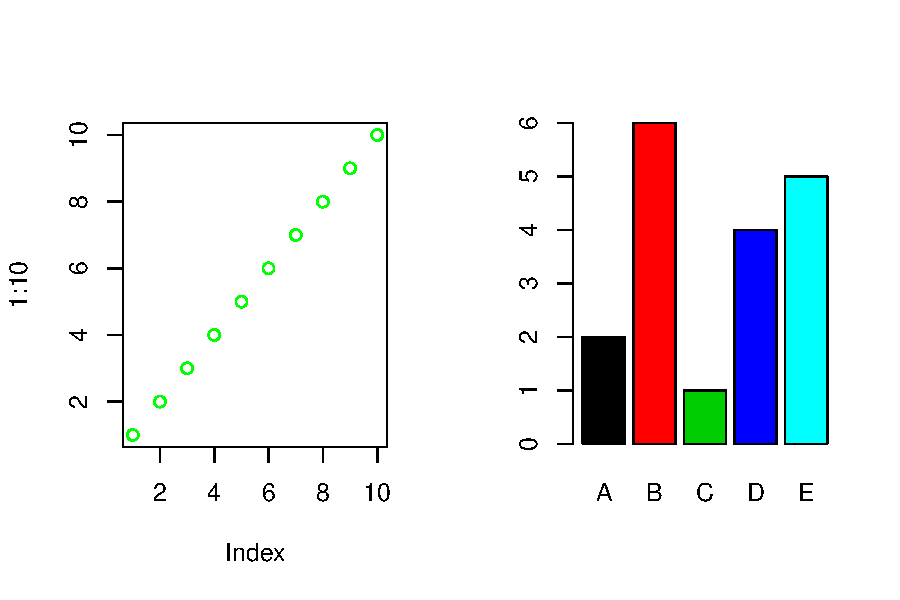
\includegraphics{Fig-test3}

\caption{Plot of 1:10 and a bar plot beside it in a figure that is 4x6 inches}

\end{figure}

\newpage
%------------------------------------
\subsection{Creating a table}
%-------------------------------------

Lets include a table using the dataset,  which is included in the default core installation of R. It contains the height and weight of 15 women.

\begin{Schunk}
\begin{Sinput}
> require(xtable)
> myTable <- summary(women)
\end{Sinput}
\end{Schunk}

We can manually encode a table in latex 


\begin{center}
\begin{tabular}{rrrrrrrr} 

$ Min.   :58.0   $&$ Min.   :115.0   $\\
$ 1st Qu.:61.5   $&$ 1st Qu.:124.5   $\\
$ Median :65.0   $&$ Median :135.0   $\\
$ Mean   :65.0   $&$ Mean   :136.7   $\\
$ 3rd Qu.:68.5   $&$ 3rd Qu.:148.0   $\\
$ Max.   :72.0   $&$ Max.   :164.0   $\\\end{tabular}
\end{center}

But it is much easier to use the package \Rpackage{xtable}. We use the function \Rfunction{require} to load the package.

\begin{Schunk}
\begin{Sinput}
> xtab <- xtable(myTable)
> print(xtab, floating=FALSE)
\end{Sinput}
% latex table generated in R 3.5.3 by xtable 1.8-4 package
% Mon Nov  4 11:56:23 2019
\begin{tabular}{rll}
  \hline
 &     height &     weight \\ 
  \hline
X & Min.   :58.0   & Min.   :115.0   \\ 
  X.1 & 1st Qu.:61.5   & 1st Qu.:124.5   \\ 
  X.2 & Median :65.0   & Median :135.0   \\ 
  X.3 & Mean   :65.0   & Mean   :136.7   \\ 
  X.4 & 3rd Qu.:68.5   & 3rd Qu.:148.0   \\ 
  X.5 & Max.   :72.0   & Max.   :164.0   \\ 
   \hline
\end{tabular}\end{Schunk}


%------------------------------------
\subsection{More on tables}
%-------------------------------------

Let make the table nice.  Lets exclude the row numbers and include a caption on the table. We can also tag the table so we reference Table~\ref{Table:women} in the text


\begin{Schunk}
\begin{Sinput}
> xtab2<-xtable(myTable, caption="Summary of women data",  label="Table:women")
> print(xtab2,include.rownames = FALSE)
\end{Sinput}
% latex table generated in R 3.5.3 by xtable 1.8-4 package
% Mon Nov  4 11:56:23 2019
\begin{table}[ht]
\centering
\begin{tabular}{ll}
  \hline
    height &     weight \\ 
  \hline
Min.   :58.0   & Min.   :115.0   \\ 
  1st Qu.:61.5   & 1st Qu.:124.5   \\ 
  Median :65.0   & Median :135.0   \\ 
  Mean   :65.0   & Mean   :136.7   \\ 
  3rd Qu.:68.5   & 3rd Qu.:148.0   \\ 
  Max.   :72.0   & Max.   :164.0   \\ 
   \hline
\end{tabular}
\caption{Summary of women data} 
\label{Table:women}
\end{table}\end{Schunk}

\newpage
%------------------------------------
%handy to include this at the end
%------------------------------------
\section{SessionInfo}
%-------------------------------------

\begin{Schunk}
\begin{Sinput}
> sessionInfo();
\end{Sinput}
\begin{Soutput}
R version 3.5.3 Patched (2019-03-11 r77184)
Platform: x86_64-apple-darwin15.6.0 (64-bit)
Running under: macOS Mojave 10.14.6

Matrix products: default
BLAS: /Library/Frameworks/R.framework/Versions/3.5/Resources/lib/libRblas.0.dylib
LAPACK: /Library/Frameworks/R.framework/Versions/3.5/Resources/lib/libRlapack.dylib

locale:
[1] en_CA.UTF-8/en_CA.UTF-8/en_CA.UTF-8/C/en_CA.UTF-8/en_CA.UTF-8

attached base packages:
[1] stats     graphics  grDevices utils     datasets  methods   base     

other attached packages:
[1] xtable_1.8-4

loaded via a namespace (and not attached):
[1] compiler_3.5.3 tools_3.5.3   
\end{Soutput}
\begin{Sinput}
> 
\end{Sinput}
\end{Schunk}

\end{document}
